\documentclass{beamer}


\usepackage{graphicx}
\usepackage{tcolorbox}
\usepackage{eurosym}


\author{Troposph'eirb V (fusée Congo)}
\title{Mini fusée}
\subtitle{EIRSPACE 2023-2024}
\institute{ENSEIRB-MATMECA}
\date{19/10/2023}


\setbeamertemplate{footline}{%
  \hfill\insertframenumber/\inserttotalframenumber
}


\begin{document}

\begin{frame}
	
	\titlepage

	\begin{figure}

		\begin{center}

			
\includegraphics[width=0.2\linewidth]{pics/eirspace.png}
		\end{center}
	\end{figure}

\end{frame}



\begin{frame}

	\tableofcontents[sectionstyle=show,subsectionstyle=show/shaded/hide,subsubsectionstyle=show/shaded/hide]
\end{frame}



\section{Equipe}

	\begin{frame}

		\begin{center}

			\Huge EQUIPE
		\end{center}
	\end{frame}


	\begin{frame}{Liste des membres}

		Les membres de l'équipe sont : 
		
		
		\begin{itemize}

			\item Louis
			\item William
			\item Jacky
			\item Ayman
			\item Shakty
			\item Damien
		\end{itemize}
	\end{frame}

	
	\begin{frame}{Répartition des taches}
		
		\begin{itemize}
			
			\item Respo théorie mathématique : William
			\item Respo Electronique : Ayman, Louis, Jacky
			\item Respo Télécom : Shakty
			\item Respo Informatique : Damien
		\end{itemize}

	\end{frame}


	\begin{frame}{Répartition actuelle}
		
		Ceux qui s'occupent de la carrosserie sont : 
		\begin{itemize}

			\item William
			\item Jacky
			\item Ayman
		\end{itemize}


		Ceux qui s'occupent de la partie élec sont :
		\begin{itemize}

			\item Louis
			\item Shakty
			\item Damien
		\end{itemize}
	\end{frame}




\section{Présentation du projet}
	
	\begin{frame}

		\begin{center}
			
			\Huge PROJET
		\end{center}
	\end{frame}
	

	\begin{frame}{Objectifs}

		\begin{block}{Choix du nom}

			Nous avons deux propositions :
			\begin{enumerate}
				
				\item choix 1 : Perséphone
				\item choix 2 : Troposph'eirb V
			\end{enumerate}
		\end{block}
		
		


		\begin{block}{Signature}

			Nous voulons insérer\_signature
		\end{block}
		
	\end{frame}


	\begin{frame}{Croquis temporaire}
		
		\begin{center}

			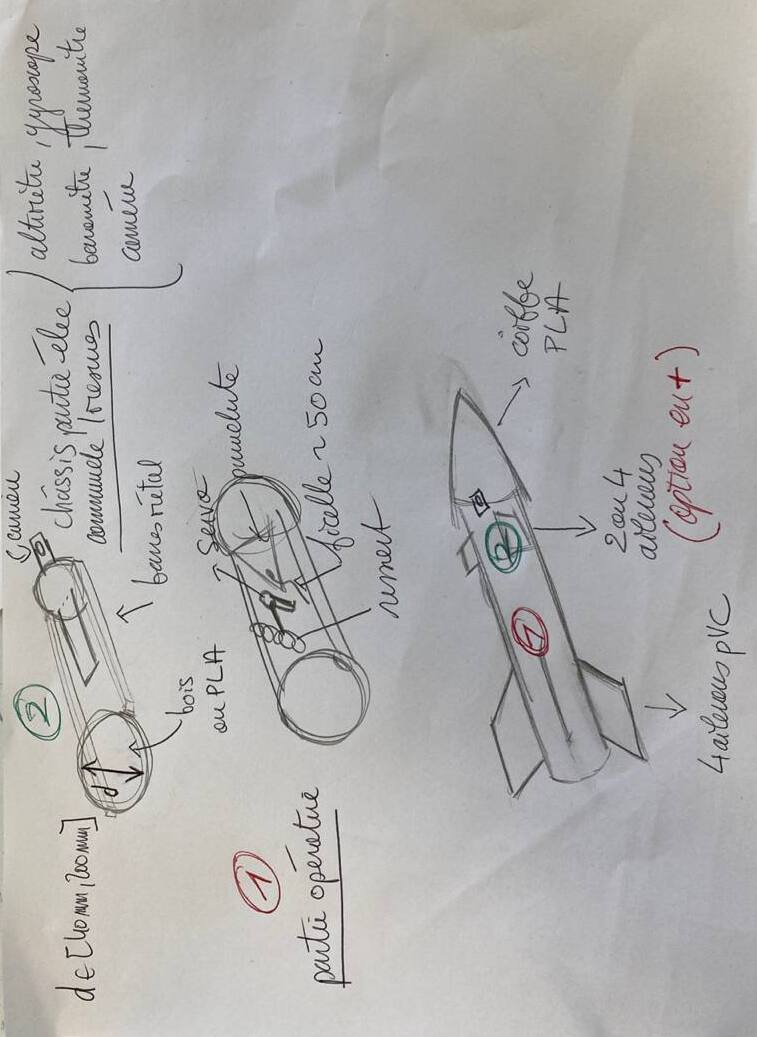
\includegraphics[width=0.6\linewidth,angle=270]{pics/5855222429968874941_121.jpg}
		 \end{center}
	\end{frame}
	
	
	\begin{frame}{Deuxième croquis}	
	
		\begin{center}	
	
			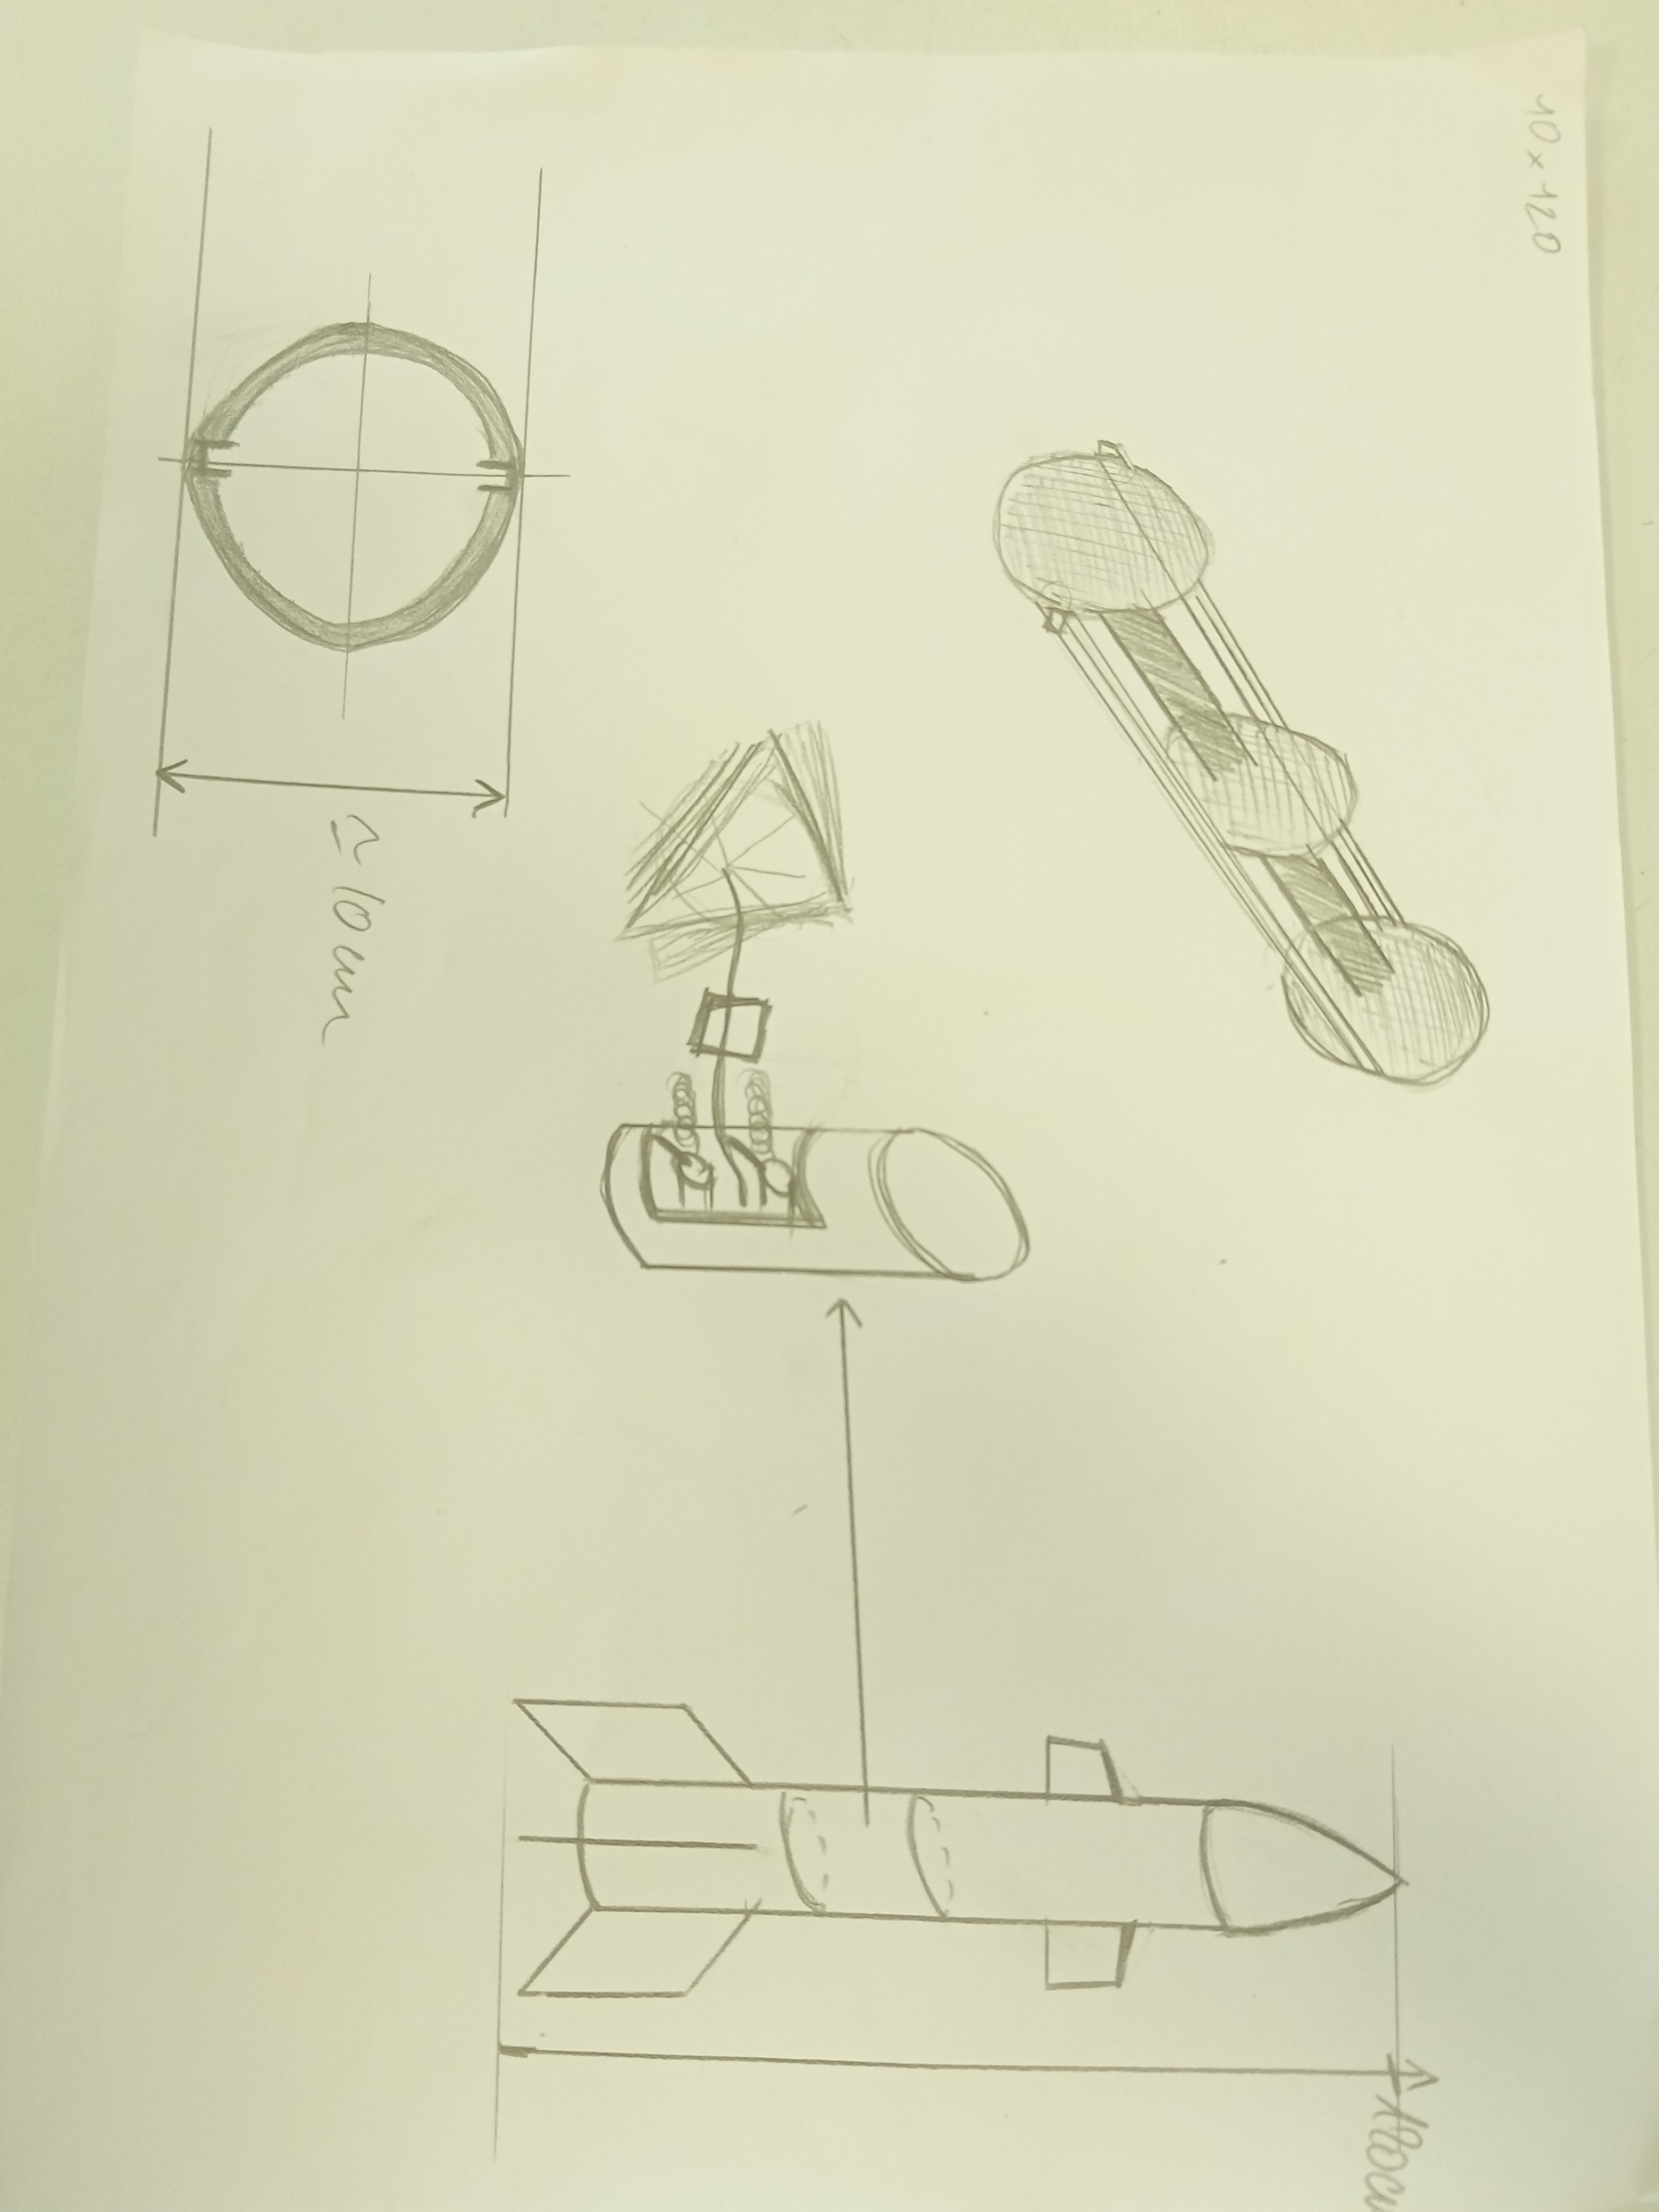
\includegraphics[width=0.7\linewidth,angle=90]{pics/croquis_2.png}
		\end{center}
	\end{frame}


	\begin{frame}{Croquis attendu}

		\begin{center}

			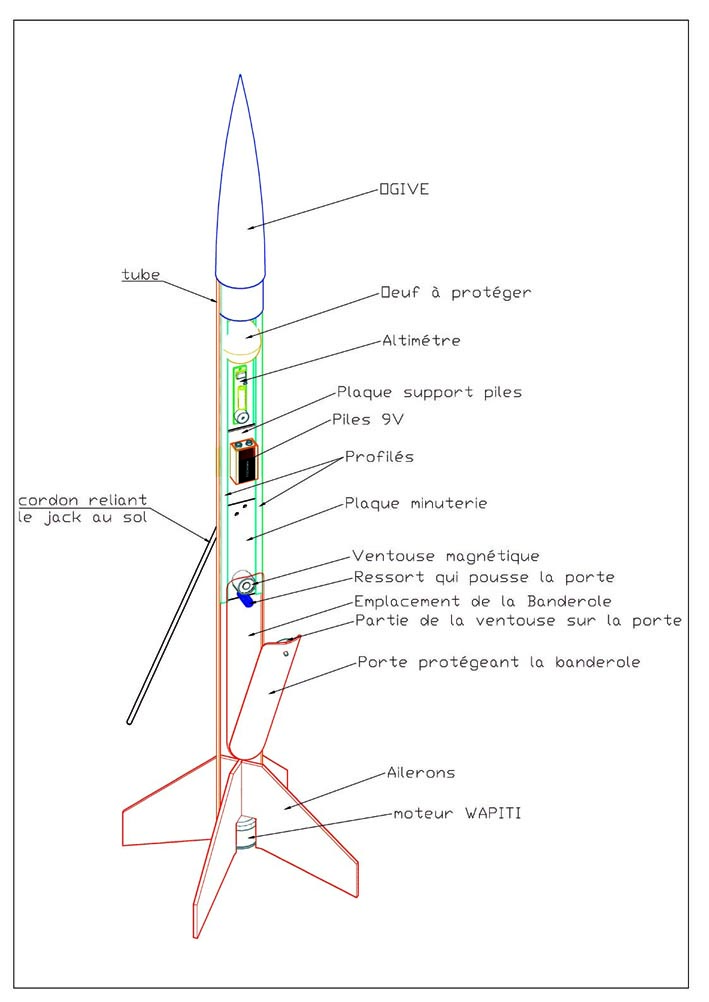
\includegraphics[width=0.5\linewidth]{pics/Minif_RC_Perspective_V4_light_web.jpg}
		\end{center}
	\end{frame}



\section{Devis provisoire}

	\begin{frame}

		\begin{center}

			\Huge DEVIS
		\end{center}
	\end{frame}

	
	\begin{frame}
		
		\frametitle{Outils nécessaires}
		\fontsize{12}{14}\selectfont

		\begin{itemize}

			\item pistolet à colle
			\item scie sauteuse
			\item potentiomètre
			\item fer à souder
			\item imprimante 3D
		\end{itemize}
	\end{frame}

	
	\begin{frame}{Matières premières}

		\fontsize{6}{12}\selectfont
		
		Pour le chassis : 

		\begin{itemize}
			
			\item 1 buche de bois, mini 10cm de diamètre
			\item 1 tube en pvc, dimensions hypothétiques : longueur=80cm, diamètre=10cm
			\item 6 barettes de métal pour la solidité du chassis (1 cm de large)			
			\item 10 tubes de colle
			\item "plastique" pour les ailerons ?, plaque de 1 $m^2$
		\end{itemize}

		
		Pour l'électronique :

		\begin{itemize}

			\item 1 altimètre
			\item 1 gyroscope
			\item 1 caméra
			\item 1 carte sd
			\item 1 servomoteur
			\item 1 carte arduino nano
			\item 1 carte réseau ?
			\item plusieurs résistances (à déterminer)
			\item 2 m de cable électrique petit diamètre
			\item 5 m d'étain
			\item 2 piles 9V
		\end{itemize}

	\end{frame}


	\begin{frame}{Matières premières}

		\fontsize{6}{12}\selectfont
		

                Pour le parachute à culmination :
                \begin{itemize}

                        \item 1 ressort
                        \item 1 corde de 50 cm
                        \item 1 parachute
                        \item idée : 1 bulle à niveau pour déclencher le parachute (donc un hydromètre aussi)
                \end{itemize}



                Pour la propulsion :

                \begin{itemize}

                        \item 1 moteur Wapiti ?
                \end{itemize}

	\end{frame}
	
	
	\begin{frame}{Estimation du prix total}
		
		\fontsize{6}{12}\selectfont

		\begin{itemize}

			\item tube en pvc : 4 \texteuro{}
			\item barettes de métal largeur 1 cm : $\leq 10$ \texteuro{}
			\item altimètre : 10 \texteuro{}
			\item gyroscope : 5 \texteuro{}
			\item carte sd : 4 \texteuro{}
			\item boitier carte sd : 2 \texteuro{}
			\item servomoteur : 10 \texteuro{}
			\item carte arduino nano : 13 \texteuro{}
			\item plusieurs résistances : $\leq 10$ \texteuro{}
			\item 1 pile 9V : 9 \texteuro{}, 2 piles 9V : 18 \texteuro{}
			\item matériau parachute : 10 \texteuro{}
		\end{itemize}


		Le total est : 96 \texteuro{}.


		Il reste donc 54 \texteuro{} de marge pour l'imprimante 3D et autre (carte réseau ?).
	\end{frame}
	

	\begin{frame}

		
	
		
	\end{frame}


\end{document}
